\documentclass[11pt, a4paper, norsk]{NTNUoving}
\usepackage[utf8]{inputenc}
\usepackage[T1]{fontenc}
\usepackage{tikz}

\ovingnr{2}    % Nummer på innlevering
\semester{Høsten 2019}
\fag{TMA 4115}
\institutt{Institutt for matematiske fag}


\begin{document}

% Kommentar

% Et felt starter ofte med \begin{<sett in kommando>}, da er det viktig å avslutte med \end{<sett in kommando>}. Det er mange eksempler på dette nedenfor!

% Du må alltid bruke $<sett inn matematikk>$, $$<sett inn matematikk>$$ eller \[<sett inn matematikk>\] for å bruke mattekommandoer.


%Dette er for enkel copy-pasting
\ifx
\begin{oppgave}
    \begin{punkt}
        \begin{align*}
        
        
        \end{align*}
    \end{punkt}
\end{oppgave}

\begin{align*} %align for å få ligninger på linje
  \begin{bmatrix}
  1 & 2 & 5\\
  3 & 4 & 6
  \end{bmatrix}
  &\sim 
  \begin{bmatrix}
  1 & 2 & 5\\
  0 & -2 & -4
  \end{bmatrix}
  
 \end{align*}

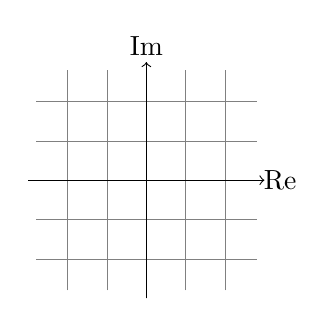
\begin{tikzpicture}
    \draw[step=.5cm,gray,very thin] (-1.4,-1.4) grid (1.4,1.4);
    \draw (-1.5,0) -- (1.5,0);
    \draw (0,-1.5) -- (0,1.5);
    \draw[->] (-1.5,0) -- (1.5,0); 
    \draw[->] (0,-1.5) -- (0,1.5);
    \draw (0, 1.7) node {Im};
    \draw (1.7, 0) node {Re};
\end{tikzpicture}
\fi

%Her begynner dokumentet
%#####################################

\begin{oppgave}
    \begin{punkt}
        I dette tilfellet er matrisen allerede redusert. Vi ser at $x_1$ og $x_4$ kan være hva som helst, ettersom de ganges med en null-kolonne. Vi setter $x_7=t$ og $x_3=s$, for $t, s \in \mathbb{C}$. Da har vi
        \begin{align*}
            &x_2+s+t = 0\\
            &x_5+t=0\\
            &x_6+t=0.
        \end{align*}
        Løsningsmengden blir da
        \begin{align*}
            \begin{bmatrix}
                x_1\\
                x_2\\
                x_3\\
                x_4\\
                x_5\\
                x_6\\
                x_7
            \end{bmatrix}=
            \begin{bmatrix}
                a\\
                -s-t\\
                s\\
                b\\
                -t\\
                -t\\
                t
            \end{bmatrix}
        \end{align*}
        for $a, b \in \mathbb{C}$ .
    \end{punkt}
    
    \begin{punkt}
    \begin{align*}
        \begin{bmatrix}
            8 & -7 & 0 & -3\\
            -8 & -7 & 3 & -7\\
            -4 & 5 & -8 & -3\\
            -6 & 6 & -4 & 0
        \end{bmatrix}
        &\sim
        \begin{bmatrix}
            8 & -7 & 0 & -3\\
            0 & -14 & 3 & -10\\
            0 & 3 & -16 & -9\\
            0 & 3 & -16 & -9
        \end{bmatrix}
        \\&\sim
        \begin{bmatrix}
            8 & -7 & 0 & -3\\
            0 & -14 & 3 & -10\\
            0 & 0 & -215 & -156\\
            0 & 0 & 0 & 0
        \end{bmatrix}
        \\&\sim
        \begin{bmatrix}
            8 & -7 & 0 & -3\\
            0 & -14 & 0 & \frac{2618}{215}\\
            0 & 0 & 215 & 156\\
            0 & 0 & 0 & 0
        \end{bmatrix}
        \\&\sim
        \begin{bmatrix}
            16 & 0 & 0 & \frac{1328}{215}\\
            0 & 215 & 0 & 187\\
            0 & 0 & 215 & 156\\
            0 & 0 & 0 & 0
        \end{bmatrix}
        \\&\sim 
        \begin{bmatrix}
            215 & 0 & 0 & 83\\
            0 & 215 & 0 & 187\\
            0 & 0 & 215 & 156\\
            0 & 0 & 0 & 0
        \end{bmatrix}
    \end{align*}
    Da har vi at 
    \begin{align*}
        \textbf{x} =\frac{1}{215}
        \begin{bmatrix}
            83\\
            187\\
            156
        \end{bmatrix}
    \end{align*}
    \end{punkt}
\end{oppgave}

\begin{oppgave}
        Egenskapen vi trenger av \textbf{u} er at den ikke er i samme plan som \textbf{v} og \textbf{w}. En slik vektor er enhetsvektoren i $x$-retning.
        
        Hvis de tre vektorene skal utspenne $\mathbb{R}^3$ så vil den eneste løsningen på likningen $x\textbf{u}+y\textbf{v}+z\textbf{w}$ være $x, y, z=0$.
\end{oppgave}

\begin{oppgave}
    \begin{punkt}
        \begin{align*}
            \begin{bmatrix}
                p(x)\\
                q(x)\\
                s(x)
            \end{bmatrix}
            = x^2
            \begin{bmatrix}
                1\\
                4\\
                1
            \end{bmatrix}
            +x 
            \begin{bmatrix}
                5\\
                18\\
                8
            \end{bmatrix}
            +
            \begin{bmatrix}
                -3\\
                4\\
                2
            \end{bmatrix}
        \end{align*}
        Vi har da tre likninger for a og b, en for hver eksponent av $x$.
        \begin{align*}
            \begin{bmatrix}
                1 & 4 \\
                5 & 18\\
                -3 & 4
            \end{bmatrix}
            \begin{bmatrix}
                a \\
                b
            \end{bmatrix}
            =
            \begin{bmatrix}
                1 \\
                8\\
                2
            \end{bmatrix}
        \end{align*}
        
        \begin{align*}
            \begin{bmatrix}
                1 & 4 & 1\\
                5 & 18 & 8\\
                -3 & 4 & 2
            \end{bmatrix}
            &\sim
            \begin{bmatrix}
                1 & 4 & 1\\
                0 & -2 & 3\\
                0 & 16 & 5
            \end{bmatrix}
        \end{align*}
        Her ser vi at vi får en motsigelse. $-2b=3$ og $16b=5$ kan ikke begge være sanne samtidig. Det finnes altså ingen $a$ og $b$ slik at $s(x) = a\cdot p(x) + b\cdot q(x)$
    \end{punkt}
    
    \begin{punkt}
        Dette er ekvivalent med at vektorene for koeffisientene til funksjonene er lineært uavhengige. Vi så i forrige oppgave at $s$ ikke var en lineær kombinasjon av de to andre. Da vil $t(x) = s(x)$ være en løsning på oppgaven. 
    \end{punkt}
\end{oppgave}

\begin{oppgave}[1]
        \begin{align*}
            A\textbf{w} &= 2A\textbf{v}_1-A\textbf{v}_2\\
            &=\begin{bmatrix}
                2\cdot 1-2 \\
                2\cdot (-1) - 3
            \end{bmatrix}
            =\begin{bmatrix}
                0 \\
                -5
            \end{bmatrix}
        \end{align*}
\end{oppgave}

\begin{oppgave}[2]
    \begin{punkt}
        Nei
    \end{punkt}
    
    \begin{punkt}
        Ikke-kvadratiske matriser har ingen entydig invers. De kan ha en høyre- og/ eller venstre-invers. Vi har ikke lært hvordan man regner ut disse enda.
    \end{punkt}
    
    \begin{punkt}
        \begin{align*}
            \left[
                \begin{array}{ccc|ccc}
                1 & 2 & 3 & 1 & 0 & 0 \\
                2 & 3 & 4 & 0 & 1 & 0 \\
                3 & 4 & 5 & 0 & 0 & 1 \\
                \end{array}
            \right]
            &\sim
            \left[
                \begin{array}{ccc|ccc}
                1 & 2 & 3 & 1 & 0 & 0 \\
                0 & -1 & -2 & -2 & 1 & 0 \\
                0 & -2 & -4 & -3 & 0 & 1 \\
                \end{array}
            \right]
        \end{align*}
        Her får vi en motsigelse. Matrisen har altså ikke en invers. 
    \end{punkt}
\end{oppgave}

\begin{oppgave}[3]
    \begin{punkt}
        La $A = \begin{bmatrix} \textbf{a}_1\\ \textbf{a}_2 \end{bmatrix}$ og $X = [\textbf{x}_1, \textbf{x}_2]$. Da er $B$ lik
        $\begin{bmatrix} \textbf{a}_1\textbf{x}_1 & \textbf{a}_1\textbf{x}_2 \\ \textbf{a}_2\textbf{x}_1 & \textbf{a}_2\textbf{x}_2 \end{bmatrix}$
        
        Vi har altså to likninger for hver vektorkomponent i $X$, og hver komponent har to ukjente, som da er ekvivalent med hvert sitt $2\times 2$ likningssystem. 
        
        Generaliseringen til $n\times n$ blir at du får $n$ $n\times n$ likningsssystemer. $n$ likningssystemer for hver vektorkomponent i $X$, og hver vektorkomponent gir $n$ likninger med $n$ ukjente.
    \end{punkt}
    
    \begin{punkt}
        I andre kolonne i $B$ har vi  $\textbf{a}_1\textbf{x}_2 = 1$ og $\textbf{a}_2\textbf{x}_2 = -1$. Det gir
        \begin{align*}
            x_{12}+x_{22}&=1\\
            x_{12}+x_{22}&=-1
        \end{align*}
        Likningen har altså ingen løsning. Dette ser vi også av at A ikke har en invers. 
    \end{punkt}
\end{oppgave}

\begin{oppgave}[4]
    \begin{punkt}
        Ettersom $BX \neq XB$ kan vi ikke sette  $AX+XB=(A+B)X$, som ville vært ekvivalent med oppgaven over. 
    \end{punkt}
    
    \begin{punkt}
        La $A=\begin{bmatrix} a_{11} & a_{12}\\ a_{21} & a_{22} \end{bmatrix}$, $B=\begin{bmatrix} b_{11} & b_{12}\\ b_{21} & b_{22} \end{bmatrix}$, $C=\begin{bmatrix} c_{11} & c_{12}\\ c_{21} & c_{22} \end{bmatrix}$, og $X=\begin{bmatrix} x_{11} & x_{12}\\ x_{21} & x_{22} \end{bmatrix}$. Da har vi
        \begin{align*}
            x_{11}a_{11}+x_{21}a_{12}+b_{11}x_{11}+b_{21}x_{12} &= c_{11}\\
            x_{12}a_{11}+x_{22}a_{12}+b_{12}x_{11}+b_{22}x_{12} &= c_{12}\\
            x_{11}a_{21}+x_{21}a_{22}+b_{11}x_{21}+b_{21}x_{22} &= c_{21}\\
            x_{12}a_{21}+x_{22}a_{22}+b_{12}x_{21}+b_{22}x_{22} &= c_{22}\\
        \end{align*}
        som er ekvivalent med
        \begin{align*}
            \begin{bmatrix}
                a_{11}+b_{11} & b_{21} & a_{12} & 0\\
                b_{12} & a_{11}+b_{22} & 0 & a_{12}\\
                a_{21} & 0 & a_{22}+b_{11} & b_{21}\\
                0 & a_{21} & b_{12} & a_{22} + b_{22}
            \end{bmatrix}
            \begin{bmatrix}
                x_{11}\\
                x_{12}\\
                x_{21}\\
                x_{22}
            \end{bmatrix}
            =
            \begin{bmatrix}
                c_{11}\\
                c_{12}\\
                c_{21}\\
                c_{22}
            \end{bmatrix}.
        \end{align*}
        Totalmatrisen er da
        \begin{align*}
            \left[
                \begin{array}{cccc|c}
                    a_{11}+b_{11} & b_{21} & a_{12} & 0 & c_{11}\\
                    b_{12} & a_{11}+b_{22} & 0 & a_{12} & c_{12}\\
                    a_{21} & 0 & a_{22}+b_{11} & b_{21} & c_{21}\\
                    0 & a_{21} & b_{12} & a_{22} + b_{22} & c_{22}
                \end{array}
            \right]     
        \end{align*}
    \end{punkt}
    
    \begin{punkt}
        Innsatt de oppgitte verdiene blir totalmatrisen slik:
        \begin{align*}
            \left[
                \begin{array}{cccc|c}
                    1 & 1 & 1 & 0 & 1\\
                    1 & 1 & 0 & 1 & 1\\
                    1 & 0 & 1 & 1 & 1\\
                    0 & 1 & 1 & 1 & 1
                \end{array}
            \right]     
            &\sim
            \left[
                \begin{array}{cccc|c}
                    1 & 1 & 1 & 0 & 1\\
                    0 & 0 & -1 & 1 & 0\\
                    0 & -1 & 0 & 1 & 0\\
                    0 & 1 & 1 & 1 & 1
                \end{array}
            \right]  
            \\&\sim
            \left[
                \begin{array}{cccc|c}
                    1 & 1 & 1 & 0 & 1\\
                    0 & -1 & 0 & 1 & 0\\
                    0 & 0 & -1 & 1 & 0\\
                    0 & 0 & 0 & 3 & 1
                \end{array}
            \right] 
            \\&\sim
            \left[
                \begin{array}{cccc|c}
                    1 & 1 & 1 & 0 & 1\\
                    0 & 3 & 0 & 0 & 1\\
                    0 & 0 & 3 & 0 & 1\\
                    0 & 0 & 0 & 3 & 1
                \end{array}
            \right] 
            \\&\sim
            \left[
                \begin{array}{cccc|c}
                    3 & 0 & 0 & 0 & 1\\
                    0 & 3 & 0 & 0 & 1\\
                    0 & 0 & 3 & 0 & 1\\
                    0 & 0 & 0 & 3 & 1
                \end{array}
            \right] 
        \end{align*}
        $X$ er altså $\frac{1}{3}\begin{bmatrix} 1 & 1\\ 1 & 1 \end{bmatrix}$.
        
    \end{punkt}
\end{oppgave}

\begin{oppgave}[1]
    $\textbf{v}_1$ og $\textbf{v}_2$ utspenner hele $\mathbb{R}^2$, så de er derfor lineært uavhengige. Om de hadde vært parallelle så hadde det ikke vært tilfellet. $\textbf{w}$-vektorene er lineært uavhengige to og to, men sammen er de lineært avhengige nettopp fordi de er lineært uavhengige to og to. Generelt utspenner $n$ lineært uavhengige vektorer $\mathbb{R}^n$, så i begge tilfellene er $\mathbb{R}^2$ utspent av vektorene.
\end{oppgave}

\begin{oppgave}
    \begin{punkt}
        \begin{align*}
            \left[
                \begin{array}{cc|c}
                   1 & 2 & 3\\
                    2 & 3 & 4\\
                    3 & 4 & 5
                \end{array}
            \right]  
            &\sim
            \left[
                \begin{array}{cc|c}
                    1 & 2 & 3\\
                    0 & -1 & -2\\
                    0 & -2 & -4
                \end{array}
            \right]
            \\&\sim
            \left[
                \begin{array}{cc|c}
                    1 & 0 & -1\\
                    0 & 1 & 2\\
                    0 & 0 & 0
                \end{array}
            \right]
        \end{align*}
        Her får vi ett pivotelement for hver kolonne. Vektorene er altså lineært uavhengige.
    \end{punkt}
    
    \begin{punkt}
        Her ser vi at $\begin{bmatrix} 2\\ 4\\ 2i \end{bmatrix} = -2i\begin{bmatrix} i\\ 2i\\ -1\end{bmatrix}$. Vektorene er lineært avhengige.
    \end{punkt}
\end{oppgave}
\begin{oppgave}[1]
    \begin{punkt}
        \begin{align*}
            det\begin{bmatrix}
            1 & 2 \\
            2 & 1
            \end{bmatrix}
            =1\cdot 1 -2\cdot 2 = -3
        \end{align*}
    \end{punkt}
    \begin{punkt}
        \begin{align*}
            det\begin{bmatrix}
            2 & -5 & 3\\
            2 & -4 & 7\\
            -6 & 15 & 1
            \end{bmatrix}
            &=2det\begin{bmatrix}
            -4 & 7\\
            15 & 1
            \end{bmatrix}
            +5det\begin{bmatrix}
            2 & 7\\
            -6 & 1
            \end{bmatrix}
            +3det\begin{bmatrix}
            2 & -4\\
            -6 & 15
            \end{bmatrix}
            \\&=2(-4-7\cdot 15) +5(2-7\cdot (-6)) +3(2\cdot 15 -(-4)\cdot (-6)
            \\&=2(-109)+5(44)+3(6)
            \\&=20
        \end{align*}
    \end{punkt}
    \begin{punkt}
        \begin{align*}
            det\begin{bmatrix}
            2i & -5 & 3\\
            2 & -4i & 7\\
            -6 & 15 & i
            \end{bmatrix}
            &=2idet\begin{bmatrix}
            -4i & 7\\
            15 & i
            \end{bmatrix}
            +5det\begin{bmatrix}
            2 & 7\\
            -6 & i
            \end{bmatrix}
            +3det\begin{bmatrix}
            2 & -4i\\
            -6 & 15
            \end{bmatrix}
            \\&=2i(4-7\cdot 15) +5(2i-7\cdot (-6)) +3(2\cdot 15 -(-4i)\cdot (-6)
            \\&=2i(-101)+5(42+2i)+3(30-24i)
            \\&=(-202i)+(210+10i)+(90-72i)
            \\&=(300-264i)
        \end{align*}
    \end{punkt}
\end{oppgave}

\begin{oppgave}[2]
    \begin{punkt}
    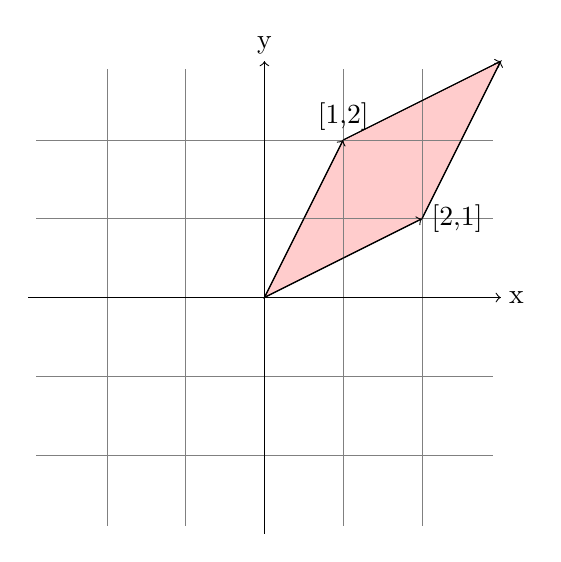
\begin{tikzpicture}
        \draw[fill=red!20] (0,0) -- (2,1) -- (3,3) -- (1,2) -- cycle;
        \draw[step=1cm,gray,very thin] (-2.9,-2.9) grid (2.9,2.9);
        \draw (-3,0) -- (3,0);
        \draw (0,-3) -- (0,3);
        \draw[->] (-3,0) -- (3,0); 
        \draw[->] (0,-3) -- (0,3);
        \draw[->] (0,0) -- (1,2) node[anchor=south]{[1,2]};
        \draw[->] (0,0) -- (2,1) node[anchor=west]{[2,1]};
        \draw[->] (1,2) -- (3,3);
        \draw[->] (2,1) -- (3,3);
        \draw (0, 3.2) node {y};
        \draw (3.2, 0) node {x};
    \end{tikzpicture}
    
    Arealet er lik absoluttverdien til determinanten, som er lik 3. 
    \end{punkt}
        \begin{punkt}
    \begin{tikzpicture}
        \draw[step=1cm,gray,very thin] (-2.9,-2.9) grid (2.9,2.9);
        \draw (-3,0) -- (3,0);
        \draw (0,-3) -- (0,3);
        \draw[->] (-3,0) -- (3,0); 
        \draw[->] (0,-3) -- (0,3);
        \draw[->] (0,0) -- (1,1) node[anchor=west]{[1,1]};
        \draw[->] (0,0) -- (2,2) node[anchor=west]{[2,2]};
        \draw (0, 3.2) node {y};
        \draw (3.2, 0) node {x};
    \end{tikzpicture}
    
    Determinanten og arealet er lik 0.
    \end{punkt}
\end{oppgave}

\begin{oppgave}[3]
    \begin{punkt}
        \begin{align*}
            det\begin{bmatrix}
            a & b & 0 & 0\\
            c & 0 & 0 & 0\\
            0 & 0 & 0 & x\\
            0 & 0 & y & z
            \end{bmatrix}
            &=-b\cdot det\begin{bmatrix}
            c  & 0 & 0\\
            0  & 0 & x\\
            0  & y & z
            \end{bmatrix}
            =-b\cdot c\cdot det\begin{bmatrix}
            0 & x\\
             y & z
            \end{bmatrix}
            \\&=bcxy
        \end{align*}
    \end{punkt}
    \begin{punkt}
        Siden $A$ er inverterbar dersom $detA \neq 0$ så er $A$ inverterbar for alle $a$ og $z$, og for alle $b, c, x, y \neq0$.
    \end{punkt}
\end{oppgave}
\end{document}